\documentclass{beamer}
\usepackage{fancyvrb}
\usepackage{hyperref}
\usepackage{tikz}
\usetikzlibrary{arrows,automata}

\usepackage{graphicx}
\newtheorem{theo}{Theorem}[section]

\newcommand{\myfig}[1]{\centerline{\includegraphics[scale=0.25]{figures/#1.png}}}

\newcommand{\trans}[5]{
\begin{tabular}{|c|c|c|c|c|}\hline
#1 & #2 & #3 & #4 & #5 \\\hline
\end{tabular}
}

\newcommand{\arr}{&\rightarrow&}
\newcommand{\darr}{&\Rightarrow&}
\newcommand{\ar}{\rightarrow}
\newcommand{\dar}{\Rightarrow}
\newcommand{\bee}{\begin{eqnarray*}}
\newcommand{\eee}{\end{eqnarray*}}
\newcommand{\emptystring}{\ensuremath{\epsilon}}

\newcommand{\bi}{\begin{itemize}}
\newcommand{\li}{\item}
\newcommand{\ei}{\end{itemize}}

\newcommand{\sect}[1]{
\section{#1}
\begin{frame}[fragile]\frametitle{#1}
}

\mode<presentation>
{
%  \usetheme{Madrid}
  % or ...

%  \setbeamercovered{transparent}
  % or whatever (possibly just delete it)
}

\usepackage[english]{babel}

\usepackage[latin1]{inputenc}

\title[Notes on Context Free Grammars]
{
Notes on Context Free Grammars
}

\subtitle{} % (optional)

\author[Geoffrey Matthews]
{Geoffrey Matthews}
% - Use the \inst{?} command only if the authors have different
%   affiliation.

\institute[WWU/CS]
{
  Department of Computer Science\\
  Western Washington University
}
% - Use the \inst command only if there are several affiliations.
% - Keep it simple, no one is interested in your street address.

\date{\today}

% If you have a file called "university-logo-filename.xxx", where xxx
% is a graphic format that can be processed by latex or pdflatex,
% resp., then you can add a logo as follows:

%\pgfdeclareimage[height=0.5cm]{university-logo}{WWULogoProColor}
%\logo{\pgfuseimage{university-logo}}

% If you wish to uncover everything in a step-wise fashion, uncomment
% the following command: 

%\beamerdefaultoverlayspecification{<+->}

\begin{document}

\begin{frame}
  \titlepage
\end{frame}


\newcommand{\myref}[1]{\small\item\url{#1}}
\newcommand{\myreft}[1]{\footnotesize\item\url{#1}}

%\begin{frame}
%  \frametitle{Outline}
%  \tableofcontents
%  % You might wish to add the option [pausesections]
%\end{frame}

\sect{Readings}

\begin{itemize}

\myreft{http://www.cs.rochester.edu/~nelson/courses/csc_173/grammars/cfg.html}

\myreft{http://en.wikipedia.org/wiki/Context-free_grammar}

\myreft{http://en.wikipedia.org/wiki/Context-free_language}
\myreft{http://en.wikipedia.org/wiki/Parsing}

\myreft{http://en.wikipedia.org/wiki/Pushdown_automata}
\myreft{http://en.wikipedia.org/wiki/LR_parser}
\myreft{https://parasol.tamu.edu/~rwerger/Courses/434/lec12-sum.pdf}
\myreft{http://www.cs.sunysb.edu/~cse350/slides/cfg3.pdf}
\end{itemize}

\end{frame}


\sect{Context Free Grammar}

A context free grammar is a grammar where all the rules are the
following form:
\[
S \rightarrow w
\]
where $S$ is a single nonterminal and $w$ is a string of terminals and
nonterminals. 

\end{frame}

\sect{Context Free Grammar Examples}


\begin{eqnarray*}
S &\rightarrow& aS | \emptystring
\end{eqnarray*}

\begin{eqnarray*}
S &\rightarrow& ABC \\
A &\rightarrow& a \\
B &\rightarrow& b\\
C &\rightarrow& c
\end{eqnarray*}

\begin{eqnarray*}
S &\rightarrow& AB | A \\
A &\rightarrow& aA | a \\
B &\rightarrow& Bb | b 
\end{eqnarray*}


\end{frame}

\sect{Context Free Grammar for Arithmetic Expressions}

\bee
E \arr T\\
E \arr E + E \\
E \arr E * E \\
E \arr (E)\\
T \arr a\\
T \arr b\\
T \arr T0\\
T \arr T1
\eee

Note that $T$ could have been reprsented by a regular language.

\end{frame}

\newcommand{\pg}[1]{\mbox{\bf\ #1\ }}
\sect{Context Free Grammar for Programming Language}
\bee
S \arr \pg{while} E \pg{do} S\ |\ \pg{if} E \pg{then} S \pg{else}
S\ |\ 
I \pg{:=} E\\
S \arr \pg{\{} SL \pg{\}} \\
L \arr SL \pg{;} | \emptystring \\
E \arr \ldots \\
I \arr \ldots
\eee
\bi
\li Reference manuals for programming languages usually give the syntax
of the language as a CFG.
\li Note that keywords, punctuation, {\em etc.}
can be represented by a regular language.
\ei
\end{frame}

\sect{Derivations}
\begin{columns}
\column{0.5\textwidth}
\bi
\li Start with $S$
\li Find a rule for a nonterminal.
\li Replace nonterminal with RHS.
\li Until no more nonterminals.
\ei
\bee
S \arr AS | \emptystring \\
A \arr AA | a\\
\eee
\[
S \dar AS \dar AAS \dar AA \dar Aa \dar aa
\]
\column{0.5\textwidth}

\myfig{derivationtree}

\centerline{Parse Tree}

\end{columns}

\vfill
\pause
The {\bf language of a grammar} is the set of all sentences for which
there exists a derivation.

\end{frame}

\newcommand{\ul}[1]{\underline{#1}}
\sect{Derivations}
\bi
\li If there is more than one possible tree for some sentence, 
the grammar is {\bf ambiguous}.
\li There are usually many possible derivations, but only one tree.
\li Important derivations are {\bf leftmost} and {\bf rightmost}.
\ei
\begin{columns}
\column{0.6\textwidth}
\bee
S \arr AS | \emptystring \\
A \arr AA | a
\eee
Rightmost:\\
\(
\ul{S} \dar A\ul{S} \dar AA\ul{S} \dar A\ul{A} \dar \ul{A}a \dar aa
\)\\
\(
\ul{S} \dar A\ul{S} \dar \ul{A} \dar A\ul{A} \dar \ul{A}a \dar aa
\)\\
Leftmost:\\
\(
\ul{S} \dar \ul{A}S \dar \ul{A}AS \dar a\ul{A}S \dar aa\ul{S} \dar aa
\)
\column{0.4\textwidth}

\myfig{derivationtree}

\centerline{Parse Tree}

\end{columns}
\bigskip
\centerline{Prove that this grammar is ambiguous.}
\end{frame}

\sect{All regular languages are context free languages}
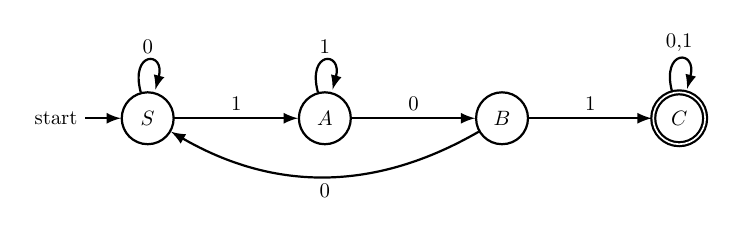
\begin{tikzpicture}[->,>=latex,thick,node distance=3cm,auto,every node/.style={scale=0.75}]
  \node[state,initial] (1) {$S$};
  \node[state] (2) [right of=1] {$A$};
  \node[state] (3) [right of=2] {$B$};
  \node[state,accepting] (4) [right of=3] {$C$};
  \path (1) edge [loop above] node {0} (1)
  (1) edge node {1} (2)
  (2) edge [loop above] node {1} (2)
  (3) edge [bend left] node {0} (1)
  (2) edge node {0} (3)
  (3) edge node {1} (4)
  (4) edge [loop above] node {0,1} (4);
\end{tikzpicture}
\bee
S \arr 0S \mid 1A \\
A \arr 0B \mid 1A \\
B \arr 0S \mid 1C \\
C \arr 0C \mid 1C \mid \emptystring
\eee

\end{frame}

\sect{Generate All Possible Sentences from a CF grammar}
\begin{columns}
\column{0.3\textwidth}
\bee
S \arr abS \ | \ bAc \ | \ d\\
A \arr aA \ | \ \emptystring
\eee
\column{0.5\textwidth}
Length 1 derivations:
\bee
S \darr abS\\
S \darr bAc\\
S \darr d\\
\eee
\column{0.2\textwidth}
\begin{enumerate}
\item $d$
\end{enumerate}
\end{columns}
\end{frame}

\sect{Generate All Possible Sentences from a CF grammar}
\begin{columns}
\column{0.3\textwidth}
\bee
S \arr abS \ | \ bAc \ | \ d\\
A \arr aA \ | \ \emptystring
\eee
\column{0.5\textwidth}
Length 2 derivations:
\bee
S \darr abS \dar ababS\\
S \darr abS \dar abbAc\\
S \darr abS \dar abd\\
S \darr bAc \dar baAc\\
S \darr bAc \dar bc\\
\eee
\column{0.2\textwidth}
\begin{enumerate}
\item  $d$
\item $abd$
\item $bc$
\end{enumerate}
\end{columns}
\end{frame}

\sect{Generate All Possible Sentences from a CF grammar}
\begin{columns}
\column{0.3\textwidth}
\bee
S \arr abS \ | \ bAc \ | \ d\\
A \arr aA \ | \ \emptystring
\eee
\column{0.5\textwidth}
Length 3 derivations:
\bee
S \darr abS \dar ababS \dar abababS\\
S \darr abS \dar ababS \dar ababbAc\\
S \darr abS \dar ababS \dar ababd\\
S \darr abS \dar abbAc \dar abbaAc\\
S \darr abS \dar abbAc \dar abbc\\
S \darr bAc \dar baAc \dar baaAc\\
S \darr bAc \dar baAc \dar bac\\
\eee
\column{0.2\textwidth}
\begin{enumerate}
\item  $d$
\item $abd$
\item $bc$
\item $ababd$
\item $abbc$
\item $bac$
\item \ldots
\end{enumerate}
\end{columns}
\end{frame}

\sect{CFG problems}
\bi
\li Any regular language.
\li $a^nb^n$
\li $a^nb^{2n}$
\li $a^nb^{3n}$
\li $a^{4n+5}b^{3n+2}$
\li $a^nb^ma^n$
\li Even length palindromes
\li Odd length palindromes
\li All palindromes
\li All strings with the same number of $a$'s and $b$'s
\li $\{a^ib^jc^k\ |\ i \not = j \mbox{~or~} j \not = k\}$
\ei
\end{frame}


\sect{Removing $\emptystring$ from grammars}

\bee
S \arr aDaE\\
D \arr bD \ | \ E\\
E \arr cE \ | \ \emptystring
\eee

\bi
\li Find all nonterminals $N$ such that $N \dar^* \emptystring$.
\li Make new rules from old by removing one or more
of the null nonterminals. 
\li Remove all null productions $N\ar \emptystring$.
\li May have to keep $S\ar \emptystring$, but only if $\emptystring \in L(S)$.
\ei


\end{frame}

\sect{Removing $\emptystring$ from grammars}
\begin{columns}
\column{0.35\textwidth}
\bee
S \arr aDaE\\
D \arr bD \ | \ E\\
E \arr cE \ | \ \emptystring
\eee

\column{0.65\textwidth}
\bi
\li Null nonterminals:  $D$ and $E$
\ei

\bigskip

\begin{tabular}{ll}
Original Production & New Productions \\\hline
$S\ar aDaE$ & $S \ar aaE\ | \ aDa \ | \ aa$\\
$D \ar bD$ & $ D\ar b$\\
$D\ar E$ & $D\ar \emptystring$\\
$E\ar cE$ & $E\ar c$\\
$E\ar \emptystring$ & none\\\hline
\end{tabular}
\bigskip

Final grammar:
\bee
S \arr aDaE \ | \ aaE \ | \ aDa\ | \ aa\\
D \arr bD \ | \ b\ | \ E\\
E \arr cE\ | \ c
\eee

\end{columns}
\end{frame}


\sect{Chomsky Normal Form}
\bi
\li All rules must be in one of these forms:
\bee
A \arr BC\\
A \arr a\\
S \arr \emptystring
\eee

\li $A$, $B$ and $C$ are nonterminals, $a$ is a single terminal, and
$S$ is the start symbol. 
\li The last rule is necessary only if the language contains $\emptystring$.
\li If a grammar is in CNF, what do we know about the tree?
\li If a grammar is in CNF, how long is a derivation?
\ei
\end{frame}



\sect{Converting to Chomsky Normal Form}
\begin{enumerate}
  \li Add $S_0$, a new start symbol, and the rule $S_0\ar S$.
  \begin{itemize}\item Only necessary if $S$ is recursive\end{itemize}
\li Eliminate $\emptystring$ rules.
\begin{itemize}\item Except possibly $S_0\ar\emptystring$\end{itemize}
\li Eliminate {\bf unit} rules, $A\ar B$:
\bi
\li Find all rules $B\ar W$, where $W$ is a string longer than one.
\li Add $A\ar W$ for all of them.
\ei
\li Fix longer rules:
\bi
\li Replace $A\ar UVWXYZ$ with
\li $A\ar UA_1$, $A_1\ar VA_2$, $A_2\ar WA_3$, $A_3\ar XA_4$, $A_4\ar YZ$.
\ei
\li For each terminal $x$, add a rule $X\ar x$ and replace all
terminals in long (length two) strings with the corresponding nonterminals.
\end{enumerate}
\end{frame}

\sect{Example converting to Chomsky Normal Form}
\footnotesize
\bee
S \arr aSb \ | \ T\\
T \arr cT \ | \ \emptystring
\eee
\vspace{-1cm}
\begin{columns}
\column{0.4\textwidth}
\bee
\mbox{Step 1:\ \ }
S_0 \arr S\\
S \arr aSb \ | \ T\\
T \arr cT \ | \ \emptystring
\eee

\bee
\mbox{Step 2:\ \ }
S_0 \arr S \ | \ \emptystring\\
S \arr aSb \ |\  ab \ | \ T\\
T \arr cT \ | \ c
\eee
\bee
\mbox{Step 3:\ \ }
S_0 \arr aSb \ |\  ab \ | \ cT \ | \ c \ | \ \emptystring\\
S \arr aSb \ |\  ab \ | \ cT \ | \ c\\
T \arr cT \ | \ c\\
\eee

\column{0.6\textwidth}

\bee
\mbox{Step 4:\ \ }
S_0 \arr aD \ |\  ab \ | \ cT \ | \ c \ | \ \emptystring\\
S \arr aD\ |\  ab \ | \ cT \ | \ c\\
D \arr Sb\\
T \arr cT \ | \ c
\eee


\bee
\mbox{Step 5:\ \ }
S_0 \arr AD \ |\  AB \ | \ CT \ | \ c \ | \ \emptystring\\
S \arr AD \ |\  AB \ | \ CT \ | \ c\\
D \arr SB\\
T \arr CT \ | \ c\\
A\arr a\\
B\arr b\\
C\arr c
\eee


\vfill
\end{columns}


\end{frame}

\sect{Note on Eliminating Unit Rules}
If we have two mutually recursive unit rules, for example in the
following grammar: 
\begin{eqnarray*}
A &\rightarrow& B | XY | UVW\\
B &\rightarrow& A | DE | FGH
\end{eqnarray*}
It doesn't hurt to eliminate both of them, so long as the remainder of
the clauses is added to each:
\begin{eqnarray*}
A &\rightarrow&  XY | UVW | DE | FGH\\
B &\rightarrow&  DE | FGH | XY | UVW
\end{eqnarray*}
Any derivation that used the two unit rules, such as
\[
A \Rightarrow B \Rightarrow A \Rightarrow B \Rightarrow FGH
\]
Can be replaced by a short-circuited version
\[
A \Rightarrow FGH
\]
\end{frame}

\sect{Consequences of Chomsky Normal Form}
\bi
\li What do all trees look like?
\li What do all derivations look like?
\li How long are the derivations?
\pause
\li There are finitely many derivations for a given string.
\li To find a parse we can exhaustively search all derivations
of this length or less.
\ei
\end{frame}

\sect{Greibach Normal Form}
\bi
\li All rules must be in one of these forms:
\bee
A \arr aB_1B_2\ldots B_n\\
S \arr \emptystring
\eee
\li $B_1B_2\ldots B_n$ is a (possibly empty) string of nonterminals.
\li The last rule is needed only if the language contains $\emptystring$.
\li There can be no left recursion.
\li What do the trees look like?
\li How long are the derivations?
\ei

\end{frame}

\sect{Converting to Greibach Normal Form}
\begin{enumerate}
\li Add $S_0$, a new start symbol, and the rule $S_0\ar S$.
\li Eliminate {\bf unit} rules, $A\ar B$.
\li Remove left recursion.
\li Eliminate $\emptystring$ rules.
\li Make substitutions as needed.
\bi\li Can be very difficult and explode to many rules.\ei
\end{enumerate}


\end{frame}
\sect{Consequences of Greibach Normal Form}
\bi
\li All derivations of a string of length $n$ have $n$ steps.
\li There are only finitely many derivations of length $n$ or less.
\li To find a parse we can exhaustively search all derivations of
length $n$ or less.
\li There exists an {\bf effective procedure} to find a parse for a CFL.
\ei 
\end{frame}



\sect{Pumping Lemma for CF Languages}
\bi
\li If a CFL is infinite, it must have recursion in it somewhere:
\bee
S \arr uNy\\
N \arr vNx \ | \ w
\eee
\li This means derivations like this are possible:

\hspace{-1cm}\mbox{$S\dar uNy \dar uvNxy \dar uvvNxxy \dar \ldots \dar uv^4Nx^4y \dar uv^4wx^4y $}

\ei
\end{frame}
\sect{Pumping Lemma for CF Languages}
\begin{theo}
If a language $L$ is context-free, then there exists some $p\geq 1$
such that any string $s$ in $L$ with $|s|\geq p$ can be written as
\[
s = abcde
\]
with substrings $a,b,c,d,e\in (V\cup\Sigma)^*$,  such that
\begin{enumerate}
\item $|bcd| \leq p$
\item $|bd| \geq 1$
\item $ab^ncd^ne$ is in $L$ for all $n\geq 0$
\end{enumerate}
\end{theo}

\end{frame}

\sect{Proof that $L = 0^n1^n2^n$ is not CF}
\bi
\li Suppose $L$ is CF, then $p$ exists as in the theorem.
\li $0^p1^p2^p \in L$ by definition.
\li From theorem, $0^p1^p0^p = abcde$ and $ab^ncd^ne \in L$ for all $n$, 
but we don't know which parts are where.
\li Case 1: $b$ or $d$ contains two different digits.
\bi
\li Then $ab^2cd^2e$ must have letters out of numerical order.
\li Then $ab^2cd^2e \not \in L$, contradiction.
\ei
\li Case 2: $b$ and $d$ each contain only one kind of digit.
\bi 
\li Then  $ab^2cd^2e$ contains more of 1 or 2 kinds of
digit, not all three.
\li Then $ab^2cd^2e \not \in L$, contradiction.
\ei
\ei
\end{frame}

\sect{Pumping Lemma exercises (some are hard)}
Show that each of the following languages is not CF.
\bi
\li $1^n$ where $n$ is prime
\li $1^m$ where $m=n^2$
\li $0^\ell 1^m2^n$ where $\ell < m < n$
\li $0^n1^n2^i$ where $i \leq n$
\li $ww$ where $w\in (0 + 1)^*$
\li $0^n1^n2^n$
\ei
\end{frame}

\sect{CF Languages are closed under union, product, and closure}
\bi
\li Let $S_1$ and $S_2$ be the start symbols for $L_1$ and $L_2$.
\li A grammar for $L_1\cup L_2$ can be constructed starting with
\[ S \ar S_1 \ | \ S_2\]
\li A grammar for $L_1L_2$ can be constructed starting with
\[ S \ar S_1S_2\]
\li A grammar for $L_1^*$ can be constructed starting with
\[ S \ar S_1S \ | \ \emptystring
\]
\ei
\end{frame}

\sect{CF languages are NOT closed under complement}
\bi
\li $L = a^\ell b^m c^n$ where either $\ell \not = m$ or $m \not = n$ is
CF 
\bi \li (exercise) \ei
\li The complement of $L$ is $a^nb^nc^n$, which is not CF
\bi \li (see previous) \ei
\ei
\end{frame}

\sect{CF languages are NOT closed under intersection}
\bi
\li $L_1 = a^mb^mc^n$ is CF 
\bi \li (exercise) \ei
\li $L_2 = a^mb^nc^n$ is CF 
\bi \li (exercise) \ei
\li $L_1 \cap L_2 = a^nb^nc^n$, which is not CF
\bi \li (see previous) \ei
\ei
\end{frame}

\sect{The intersection of a CF language and a regular language is CF}
\bi
\li Given a PDA for one and a DFSA for the other:
\li Create a new PDA with states that are the cross product of the
states of the two machines.
\li As input is processed, run both machines in parallel.
\li Accept if both accept.
\ei
\end{frame}

\end{document}
